\section{El surgimiento del serialismo integral}\label{ch:serialismo}
	\subsection{Alban Berg y Anton Webern: la Segunda Escuela de Viena}
	\label{berweb}
	Adem\'as de Schoenberg, hubo dos compositores m\'as que contribuyeron al desarrollo del dodecafonismo y que demostraron con sus diferentes estilos la versatilidad del sistema. \'Estos fueron los disc\'ipulos de Schoenberg: Alban Berg y Anton Webern. 
	
	El maestro y sus dos alumnos formaron la autodenominada Segunda Escuela de Viena, llamada as\'i en honor a los miembros de la Primera: Haydn, Mozart y Beethoven. Aparte del hecho de que Schoenberg, Berg y Webern nacieron y se formaron en Viena, el nombre tambi\'en simboliza su autoproclamaci\'on como herederos leg\'itimos de la tradici\'on musical alemana proveniente del siglo XVIII.
	
	La Segunda Escuela de Viena form\'o parte de las vanguardias art\'isticas europeas, opuestas a la tendencia neocl\'asica de Stravinsky o Prokofiev. Los tres integrantes siguieron carreras compositivas similares en cuanto a estilo y concepci\'on art\'istica: una \'epoca tonal, una ruptura atonal y un desarrollo dodecaf\'onico.
	
	Con el ascenso del nazismo, Schoenberg, que era jud\'io, se vio obligado a exiliarse a Estados Unidos. Sus disc\'ipulos se quedaron en Austria, pero pasaron penurias econ\'omicas debido a la censura impuesta por el gobierno: la m\'usica dodecaf\'onica se descalific\'o como \emph{Entartete Kunst}~\cite{entartete} (``arte degenerado'').
	
	Alban Berg se centr\'o en la efusi\'on emocional y el inter\'es por lo humano, utilizando el m\'etodo dodecaf\'onico libremente y acerc\'andose a formatos tonales. Su etapa atonal fue especialmente relevante, ya que compuso entonces su primera obra dram\'atica, \href{https://www.youtube.com/watch?v=rHFFPyU41_0}{Wozzeck} (1925). Es una \'opera basada en la pieza teatral de Georg B\"uchner, en la cual Berg plasm\'o parte de sus propias experiencias como soldado en la Primera Guerra Mundial. Su segunda \'opera, \href{https://www.youtube.com/watch?v=bLuLsFjnCjI}{Lul\'u}, qued\'o inconclusa debido a su muerte por septicemia en 1935, a los 50 a\~nos.
	
	\begin{figure}[h]
		\begin{center}
			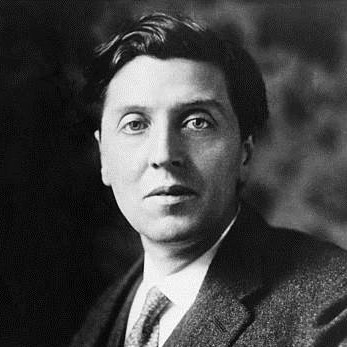
\includegraphics[width=5cm]{Alban_Berg.jpg}\\
			\caption{Alban Berg (1885\textemdash1935); figura tomada de \href{https://www.dw.com/pt-br/berg-concerto-para-violino/a-4219906}{Deutsche Welle}.}
		\end{center}
	\end{figure}
	
	Anton Webern fue un compositor m\'as riguroso en cuanto a las formas, siempre leal al sistema dodecaf\'onico y a su maestro. Se deleitaba en los procedimientos formales m\'as sutiles, aquellos que solo pod\'ian ser descubiertos al estudiar detenidamente la obra. Esto qued\'o reflejado en su dodecaf\'onico \href{https://www.youtube.com/watch?v=BqFetTU05wE}{Concierto para 9 instrumentos}, Op. 24 (1934), cuya serie est\'a construida por segmentos derivados de las tres primeras notas de la obra. Adem\'as, muestra tendencias a asignar duraciones, timbres y articulaciones a segmentos aislados, lo que m\'as tarde inspirar\'ia el serialismo integral.
        
	Durante la ocupaci\'on de Viena, Webern sali\'o de su casa una noche tras el toque de queda, y un soldado norteamericano, probablemente en estado de embriaguez, lo mat\'o a tiros. As\'i, Schoenberg, el maestro y el m\'as mayor de los tres, sobrevivi\'o a sus dos alumnos exiliado en Estados Unidos.
    
	\subsection{La escuela de Darmstadt}
	Tras la Segunda Guerra Mundial, el mundo art\'istico estaba totalmente destruido. La violencia, la censura y la incomunicaci\'on hab\'ian impedido cualquier posible desarrollo creativo, y los artistas de la generaci\'on anterior se hab\'ian aislado, exiliado o hab\'ian fallecido. Volver a construir los pilares del arte era el cometido de la nueva generaci\'on de artistas, quienes compart\'ian la sensaci\'on de que el mundo hab\'ia renacido tras la tragedia.
	
	En 1946 se crearon los Cursos de Verano de Darmstadt, fundados por Wolfgang Steinecke y patrocinados por las fuerzas americanas, con el objetivo de retomar la actividad musical en la Alemania de la posguerra. Se centraron en dar a conocer las t\'ecnicas compositivas de las generaciones anteriores. Aunque el primer a\~no estuvo enfocado en el movimiento neocl\'asico, fue en los a\~nos posteriores cuando se desarroll\'o un mayor inter\'es por las t\'ecnicas serialistas.
	
	Los cursos resultaron en la aparici\'on de una nueva escuela de compositores cuya finalidad art\'istica era crear un lenguaje musical distinto y alejado de la tradici\'on para, de esta forma, obtener una mayor libertad compositiva. Como dijo Karlheinz Stockhausen:
	
	\begin{quote}
		\textit{Los m\'etodos nuevos cambian la experiencia, y las experiencias nuevas cambian al hombre.}\\
		{\footnotesize Stockhausen en el documental autobiogr\'afico \textit{Tuning In}~\cite{stockhausen}.}
	\end{quote}
	
	Esta escuela tom\'o el nombre de la ciudad donde se realizaban los cursos: se llam\'o la Escuela de Darmstadt. El t\'ermino fue acu\~nado por el compositor Luigi Nono en una de sus clases magistrales en 1957, y con \'el se describ\'ia a s\'i mismo y a sus compa\~neros compositores: Pierre Boulez, Karlheinz Stockhausen y Bruno Maderna. Para estos compositores, la tradici\'on art\'istica estaba demasiado relacionada con los fracasos pol\'iticos y las penurias sociales pasadas, y precisamente por ello cre\'ian necesario romper con todos los v\'inculos heredados.
    Sin embargo, para crear aquel nuevo lenguaje no tomaron como referencia el dodecafonismo de Schoenberg, ya que \'el ve\'ia su sistema como parte de la tradici\'on musical, como un elemento m\'as en la evoluci\'on de la m\'usica. Se centraron, en cambio, en la formalidad y abstracci\'on del serialismo de Anton Webern, y desarrollaron a partir de sus m\'etodos el denominado \textbf{serialismo integral}.
    
    \begin{figure}[h]
    	\begin{center}
    		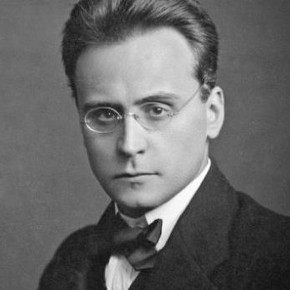
\includegraphics[width=5cm]{Anton_Webern.jpg}\\	
    		\caption{Anton Webern (1883\textemdash1945); figura tomada de \href{https://www.francemusique.fr/personne/anton-webern}{France Musique}.}
    	\end{center}
    \end{figure}

    Para la Escuela de Viena el estilo compositivo de Webern era tan solo un posible enfoque del amplio abanico que abarcaba el dodecafonismo, pero en Darmstadt se consider\'o un avance de \'este.
	
	El \textbf{serialismo integral} es un sistema de composici\'on musical que predetermina los materiales compositivos \textemdash la melod\'ia, la armon\'ia, el ritmo, el timbre\textemdash~a partir de la ordenaci\'on serial de los diferentes par\'ametros musicales: alturas, intensidades, duraciones, ataques o instrumentos, entre otros. 
	
	Es un desarrollo del serialismo dodecaf\'onico de Schoenberg, que serializa solamente las alturas, hacia los dem\'as par\'ametros sonoros. Tiene, por tanto, un alto grado de planificaci\'on pre-composicional: se pretende que la determinaci\'on compositiva sea absoluta; y se tiende al automatismo del arte y sus formas, alej\'andolo de cualquier evocaci\'on decimon\'onica.

	Desde sus comienzos, el serialismo integral suscit\'o numerosas cr\'iticas, incluso desde el propio colectivo vanguardista. Una de ellas fue la falta de elecci\'on del int\'erprete a la hora de transmitir la obra. El int\'erprete serialista debe reproducir con total exactitud cada detalle de la partitura, y, por tanto, no puede aportar car\'acter alguno. 
	
	Otra de las cr\'iticas m\'as extendidas fue la incapacidad para interpretar estas obras correctamente debido a su complejidad t\'ecnica. Adem\'as, los detalles que precisamente las hacen complejas son, en su mayor parte, inapreciables por parte del oyente.
	
	\subsection{Pierre Boulez}
	\label{boulez}
    El compositor que cre\'o y utiliz\'o por primera vez el serialismo integral, adem\'as de instruirlo y difundirlo a los dem\'as compositores de Darmstadt, fue el compositor franc\'es Pierre Boulez. Otros m\'usicos hab\'ian compuesto obras con tendencias serialistas y elementos predeterminados, como Olivier Messiaen en \href{https://www.youtube.com/watch?v=Rz_KRRqvID4}{\emph{Mode de valeurs et d'intensit\'es}}, pero fue Boulez quien sent\'o sus bases y su t\'ecnica. De hecho, los compositores precedentes influyeron prominentemente en la m\'usica de Boulez gracias a las clases impartidas en los cursos de Darmstadt.
    
    \begin{figure}[h]
    	\begin{center}
    		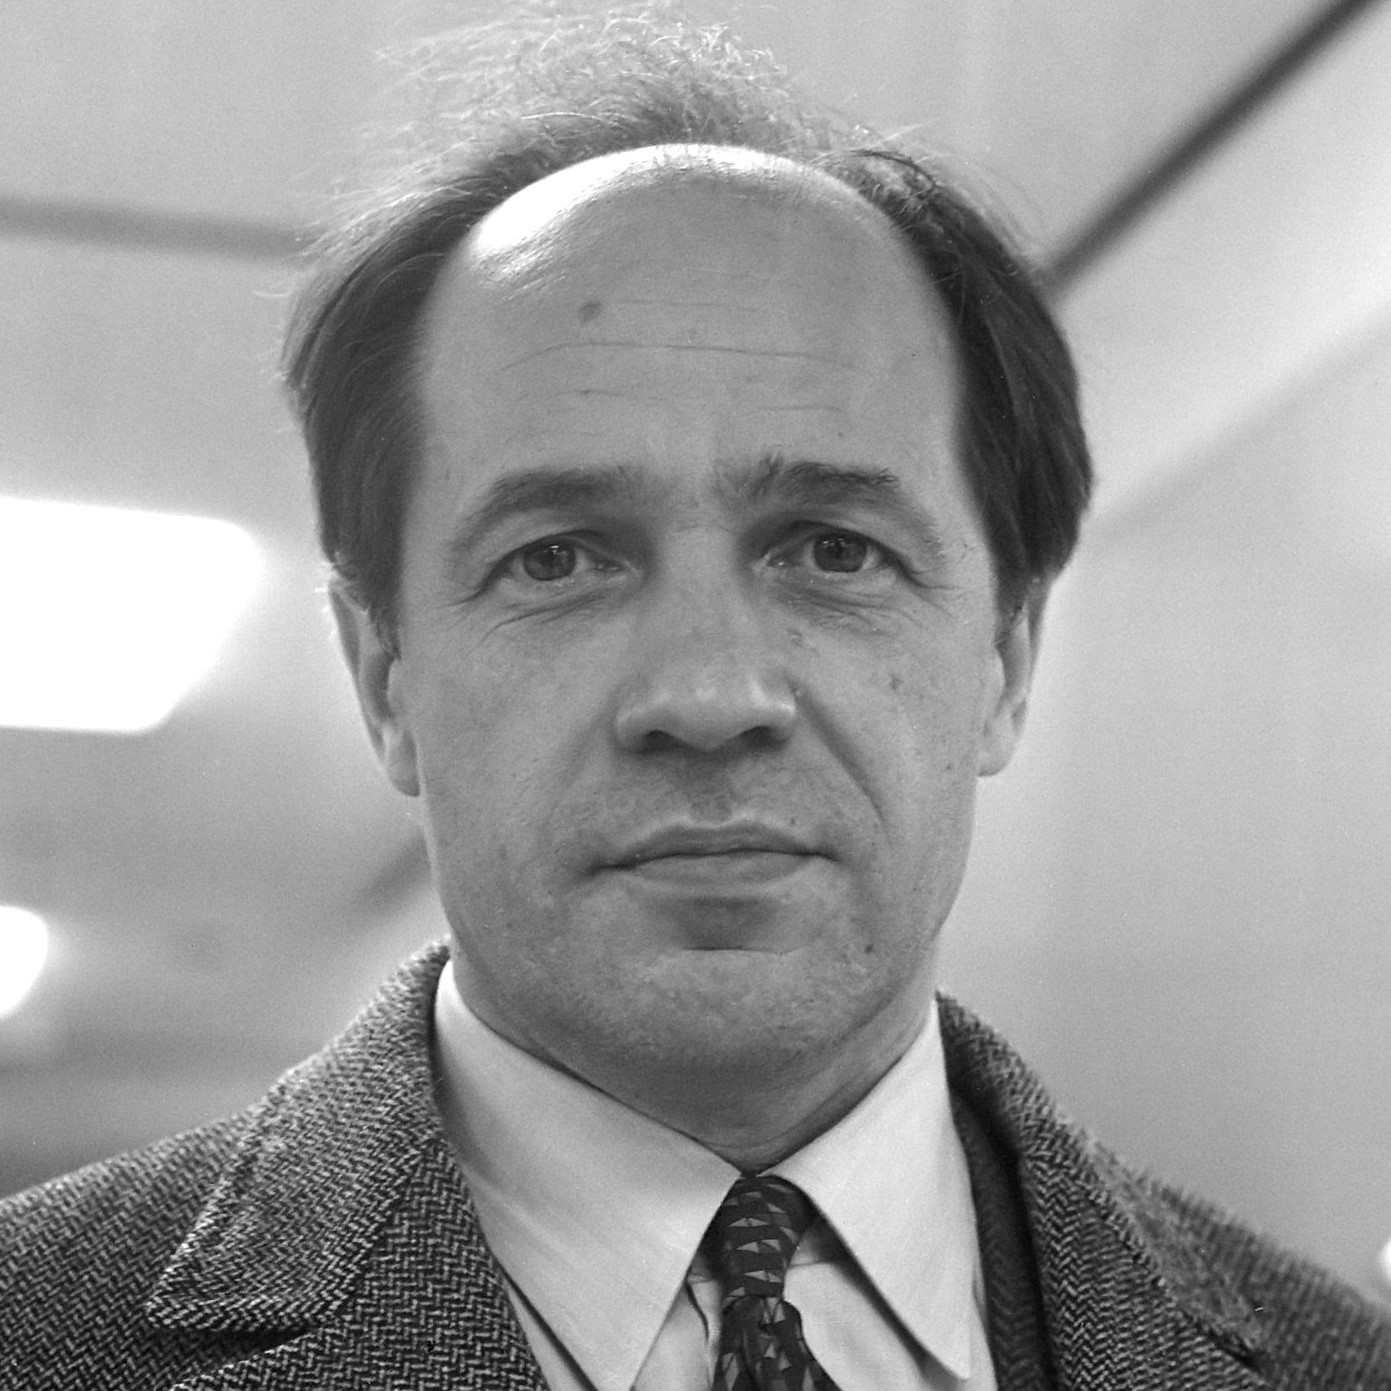
\includegraphics[width=5cm]{Pierre_Boulez.jpg}\\
    		\caption{Pierre Boulez (1925\textemdash2016); figura tomada de \href{http://kultur-im-radio.de/blog/pierre-boulez-ich-bin-ein-wiener}{Kultur im Radio}.}
    	\end{center}
    \end{figure}
    
    Boulez consideraba necesaria y evidente la extensi\'on de elementos a predeterminar m\'as all\'a de la melod\'ia, y le parec\'ia incoherente el sistema dodecaf\'onico de Schoenberg, que para \'el estaba incompleto. En su controvertido ensayo \emph{Schoenberg ha muerto}~\cite{boulez}, publicado un a\~no despu\'es de la muerte del compositor, coment\'o:
    
    \begin{quote}\emph{En primer lugar, la exploraci\'on del campo serial ha sido conducida unilateralmente: all\'i falta el plano r\'itmico, e incluso el plano sonoro propiamente dicho: las intensidades y los ataques.} [$\ldots$] 
    	
    \emph{Pero la causa esencial de su fracaso reside en el desconocimiento profundo de las FUNCIONES seriales propiamente dichas, las funciones engendradas por el principio mismo de la serie.}\end{quote}
    
	Es decir, que para ampliar el concepto de serialismo se deb\'ia primeramente conocer el fundamento matem\'atico de las series y sus funciones transformativas. Adem\'as de ser m\'usico y compositor, Boulez hab\'ia estudiado matem\'aticas, lo que le llev\'o a querer analizar matem\'aticamente el sistema compositivo y generalizarlo para series de longitudes arbitrarias. Para \'el, el serialismo no deb\'ia ser un mero recurso compositivo, sino la ley que rige todos los elementos de la obra. De hecho, m\'as adelante en su ensayo declar\'o:
    
    \begin{quote}[\ldots] \emph{desde el descubrimiento de la Escuela de Viena, todo compositor alejado de los experimentos seriales ha resultado in\'util.}\end{quote}

	Su obra \href{https://www.youtube.com/watch?v=QUF3XPTIlJo}{\emph{Structures I}} (1952), para dos pianos, fue compuesta siguiendo las t\'ecnicas de serialismo integral: tiene series de doce alturas, doce ataques, doce duraciones y doce tipos din\'amicos, aunque m\'as tarde reducir\'ia algunas a diez.